\documentclass{beamer}
\usepackage[english]{babel}
\usepackage[latin1]{inputenc}
\usepackage[T1]{fontenc}
\usepackage{amssymb}
\usepackage{amsmath}
\usepackage{booktabs}
\usepackage{verbatim}
\usepackage{caption}
\usepackage{float}
\usepackage{csquotes}
\usepackage{sansmathaccent}
\usepackage{subfigure}
\usepackage{multicol}
\pdfmapfile{+sansmathaccent.map}
\def \ourFigPath {../../} 
\def \ourTablePath {../../Tables/} 

\setbeamersize{text margin left=5mm,text margin right=12mm} 
%
\font\reali=msbm10 at 12pt
% subsets of real numbers
\newcommand{\numberset}{\mathbb}
\newcommand{\real}{\hbox{\reali R}}
\newcommand{\N}{\numberset{N}}
\newcommand{\realp}{\hbox{\reali R}_{\scriptscriptstyle +}}
\newcommand{\realpp}{\hbox{\reali R}_{\scriptscriptstyle ++}}
\newcommand{\virgolette}[1]{``#1''}
%

\author[Brianti, Gati]{Marco Brianti and Laura Gati}

\institute[Boston College]{Boston College}


\title{IT Spillovers in TFP }

\date{\today}

\usetheme{Warsaw}


\begin{document}


\begin{frame}

\maketitle


\end{frame}

%%%%%%% Slide %%%%%%
\begin{frame}
\frametitle{Topics of today's discussion}

\begin{enumerate}
\item Model solution related questions. 

\begin{itemize}
	\item How should be $Ef_x$?
	\item Is the first partial derivative times the related state or just the first partial derivative?
	\end{itemize}

\

\item Constructing a conceptually correct GDP and TFP.

\

\item Initial results for the VECM.

\

\item Different identification procedures and their correlations.
\end{enumerate}


\end{frame}
%%%%%%%%%%%%%%%%%


%%%%%%% Slide %%%%%%
\begin{frame}
\frametitle{(2) Constructing a conceptually correct GDP and TFP}

Oulton (2010) defines GDP as follows
$$
\hat{GDP} = (1 - w) \hat{y_c} + w \hat{y_i} \ \ \ \text{where} \ \ \ w = \frac{p y_i}{y_c + p y_i}
$$
\begin{itemize}
	\item Can we use $w$ in s.s.?
\end{itemize}

\

\


Moreover, 


$$
\hat{TFP} = (1 - w) \hat{TFP_c} + w \hat{TFP_i} 
$$


\end{frame}
%%%%%%%%%%%%%%%%%



%%%%%%% Slide %%%%%%
\begin{frame}
	\frametitle{(3) VECM}

Number of cointegrating vectors is 1 as indicated by Johansen's trace test.

\

\


Identification strategy: rotation of shocks that maximizes the impact effect on IT investment s.t. a 0 impact response on TFP.	


\end{frame}
%%%%%%%%%%%%%%%%%

%%%%%%% Slide %%%%%%
\begin{frame}
\frametitle{(3) VECM}

\vspace{-0.2cm}
\begin{figure}
	\begin{multicols}{2}
		\centering 
		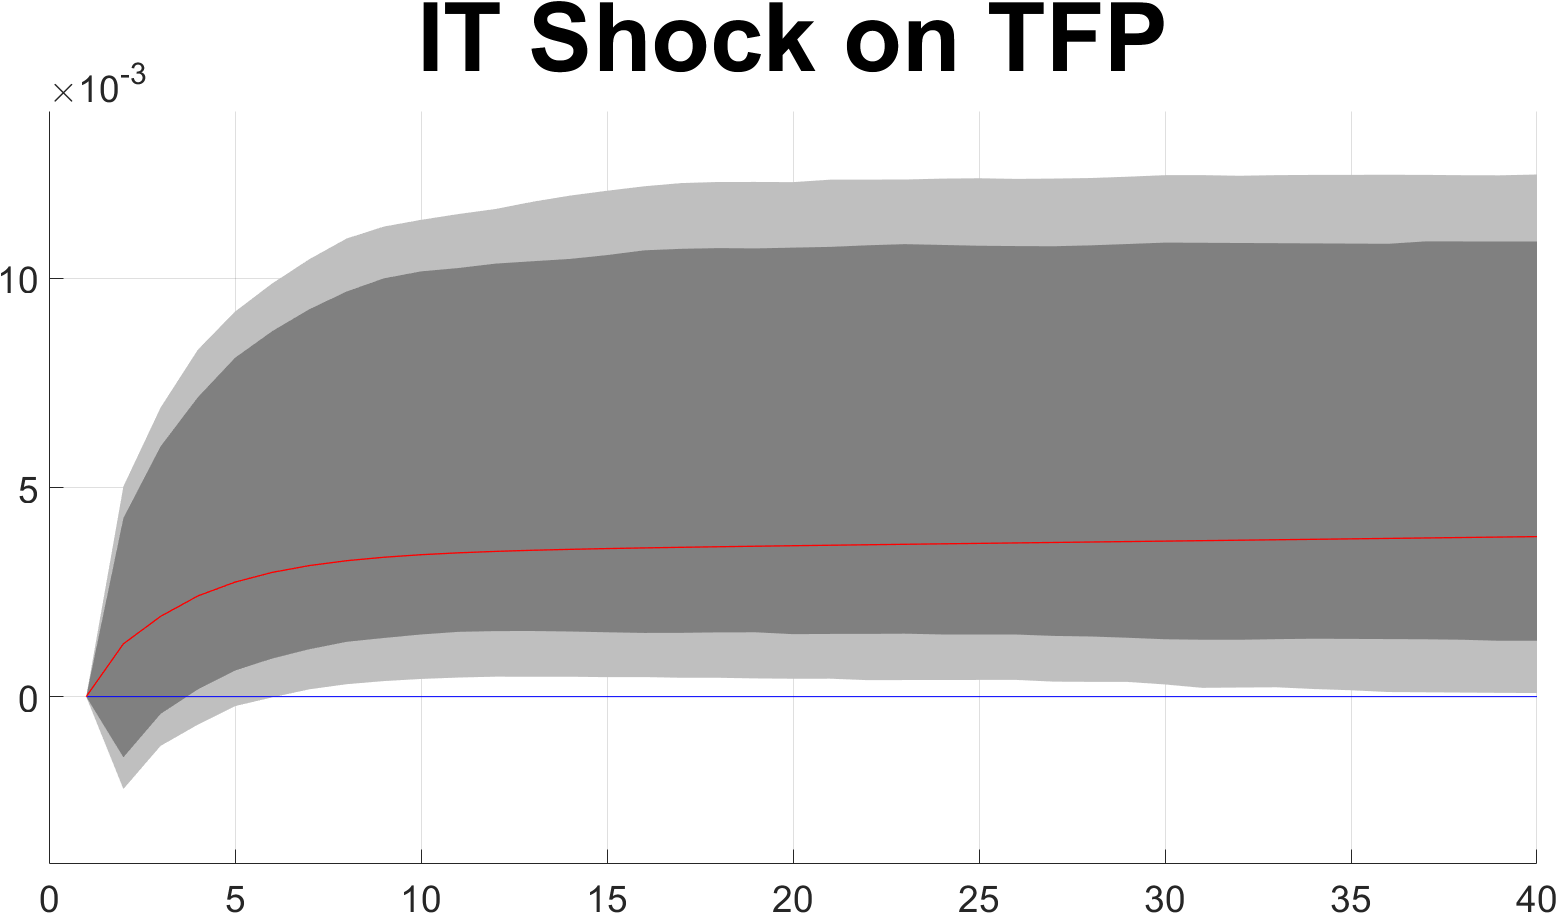
\includegraphics[scale = 0.13]{\ourFigPath Figures/fig_IT_Shock_on_TFP__JustIT_VECM}\\
		\vspace{0.3cm}
		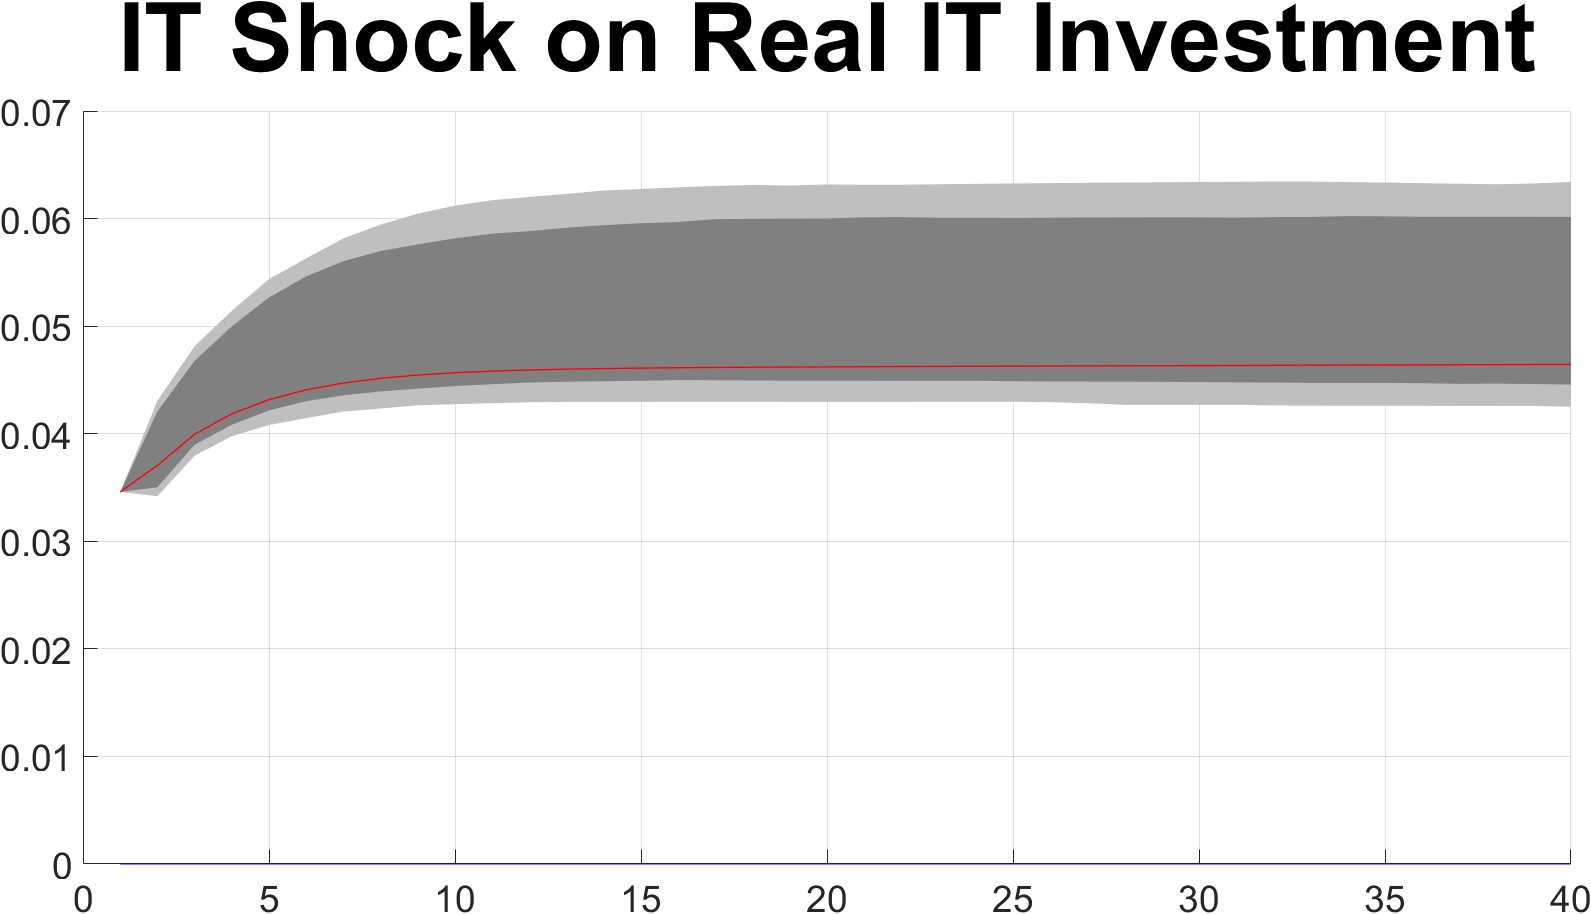
\includegraphics[scale = 0.13]{\ourFigPath Figures/fig_IT_Shock_on_Real_IT_Investment__JustIT_VECM}\\ 
		\vspace{0.3cm}
		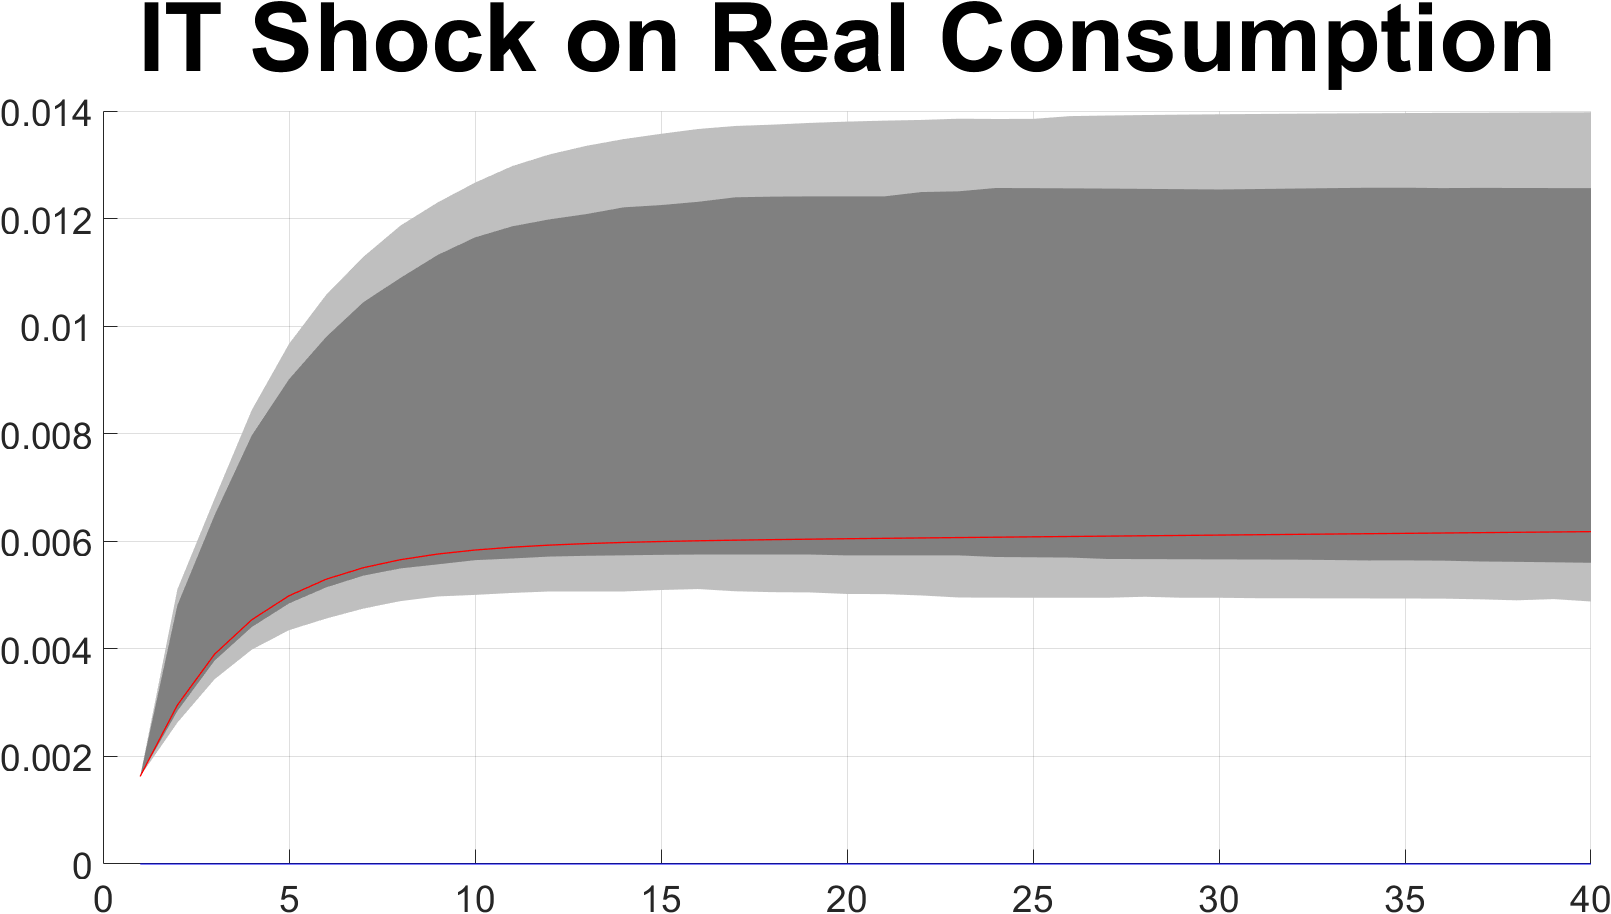
\includegraphics[scale = 0.13]{\ourFigPath Figures/fig_IT_Shock_on_Real_Consumption__JustIT_VECM}\\ 
		\vspace{0.3cm}
		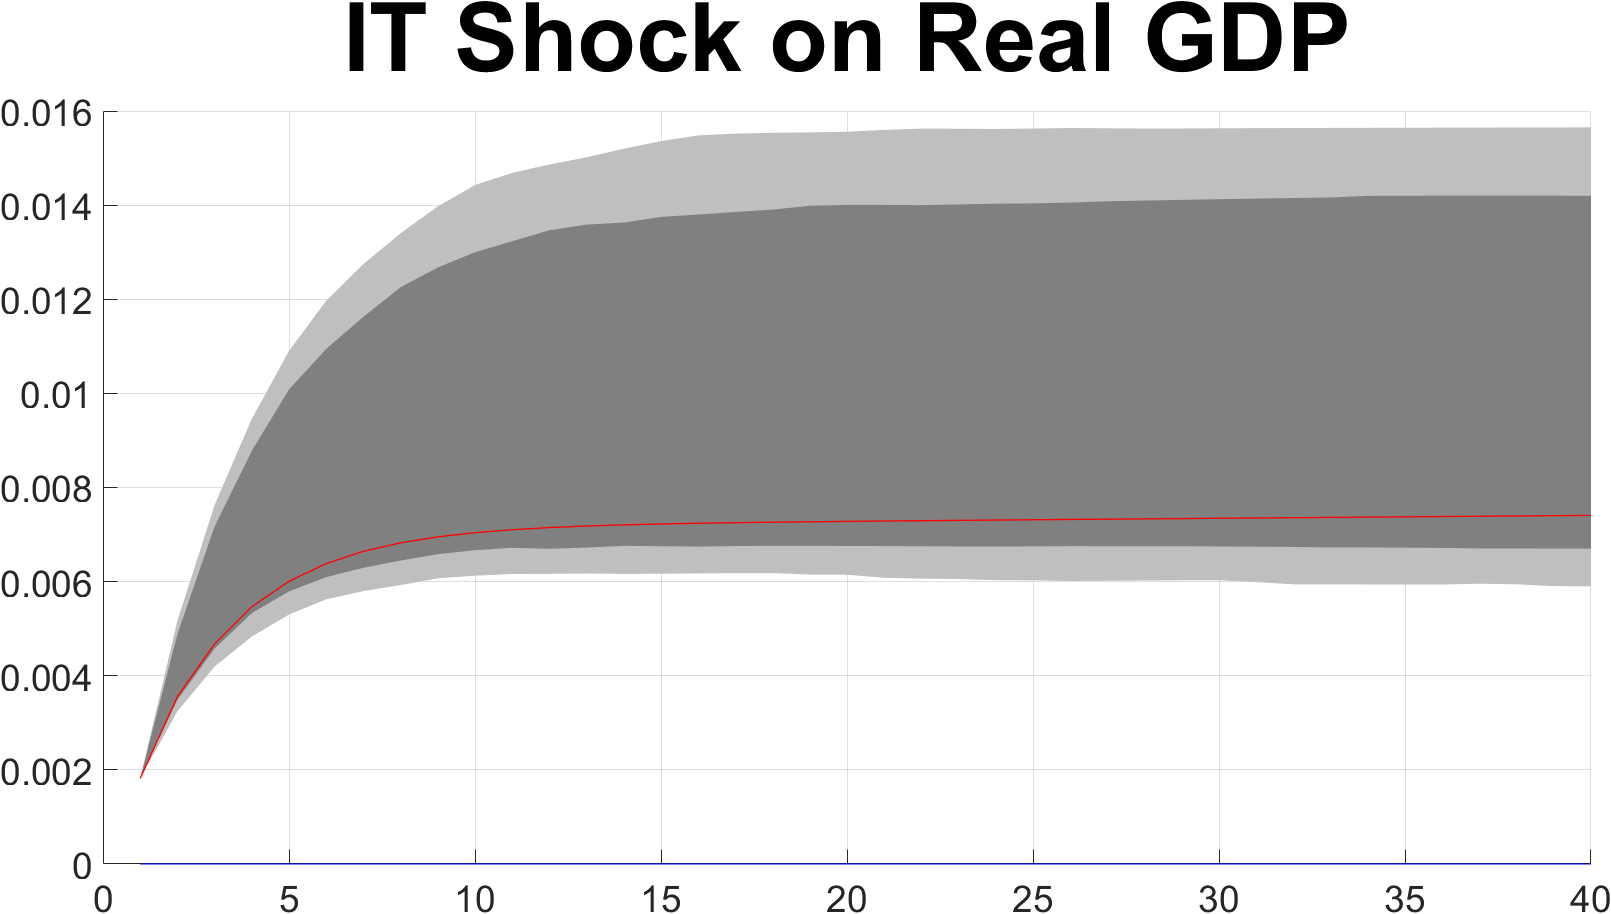
\includegraphics[scale = 0.13]{\ourFigPath Figures/fig_IT_Shock_on_Real_GDP__JustIT_VECM}\\ 
		
	\end{multicols}
\end{figure}


\end{frame}
%%%%%%%%%%%%%%%%%


%%%%%%%        Slide    %%%%%%%%%%%%%%%%%%
\begin{frame}
\frametitle{(4) Different identification procedures and their correlations.}

Two step-identification procedure.

\


\begin{enumerate}
\item Identify the news shock a la Barsky-Sims subject to some constraint suggested by the theoretical model.


\begin{itemize}
	\item Limiting the response of relative prices to a news shock.
	\item Zero-impact response of IT to a news shock.
\end{itemize}

\


\item Identify the IT shock as the one that maximizes the impact effect on IT investment s.t. a 0 impact response on TFP.
\end{enumerate}

\


\textbf{Note.} This is the only identification procedure you have not seen so far. 




\end{frame}

%%%%%%%%%%%%%%%%%%%%%%%%%

%%%%%%%        Slide    %%%%%%%%%%%%%%%%%%
\begin{frame}
\frametitle{Quick overview of identification procedures}
	\begin{enumerate}
		\item ``Old news" identification: Identify news shock and IT shock a la Barsky \& Sims, s.t. a 0 on relative prices.
		\item ``just IT" identification: identify an IT shock only as a rotation of shocks that maximizes the impact effect on IT investment s.t. a 0 impact effect on TFP.
		\item ``two-step just IT'': the new one presented above. 
	\end{enumerate}
\end{frame}


%%%%%%%%%%%%%%%%%%%%%%%%%


%%%%%%%        Slide    %%%%%%%%%%%%%%%%%%
\begin{frame}
\frametitle{Structural shock series}
\begin{center}
\begin{tabular}{ccc}
	S.1 & S.2 & S.3 \\
	1.0000   & 0.6392 &   0.6180 \\
	0.6392  &  1.0000 &   0.8359 \\
	0.6180  &  0.8359 &   1.0000 \\
\end{tabular}
\end{center}



\end{frame}


%%%%%%%%%%%%%%%%%%%%%%%%%

%%%%%%%        Slide    %%%%%%%%%%%%%%%%%%
\begin{frame}
\frametitle{Correlations}


\begin{center}
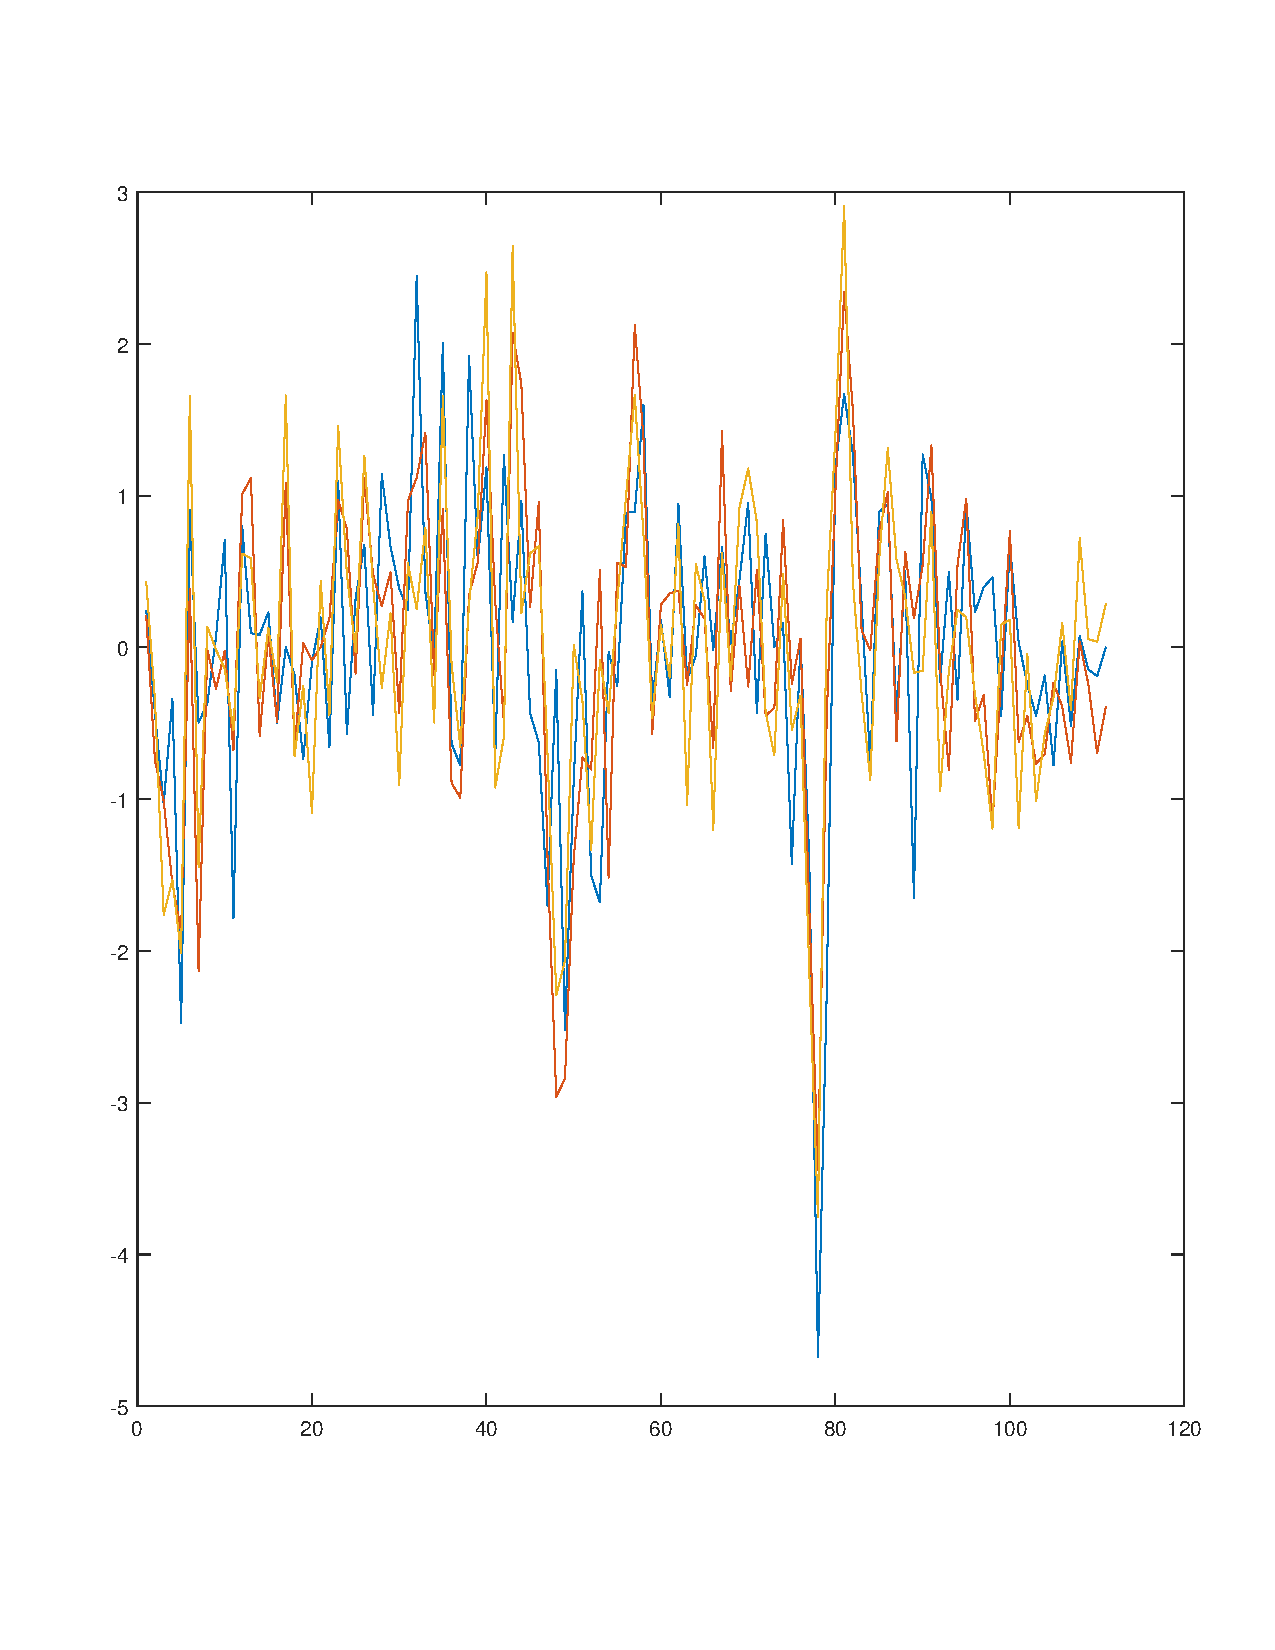
\includegraphics[scale = 0.3]{\ourFigPath Figures/structural_shocks_together}\\
\end{center}


\end{frame}


%%%%%%%%%%%%%%%%%%%%%%%%%










\end{document}
